\section{Demonstration overview}

In this section, we describe different kinds of scenarios that users commonly encountered in the Crowdrebate platform, which include a new request submission, the view of top deals and products, status checking, and data analyses.

\subsection{Scenarios 1: Set up request}

\begin{figure}[t!] \vspace{-1.5ex}
	\subfigure[][{Set up a request}]{
		\scalebox{0.09}[0.09]{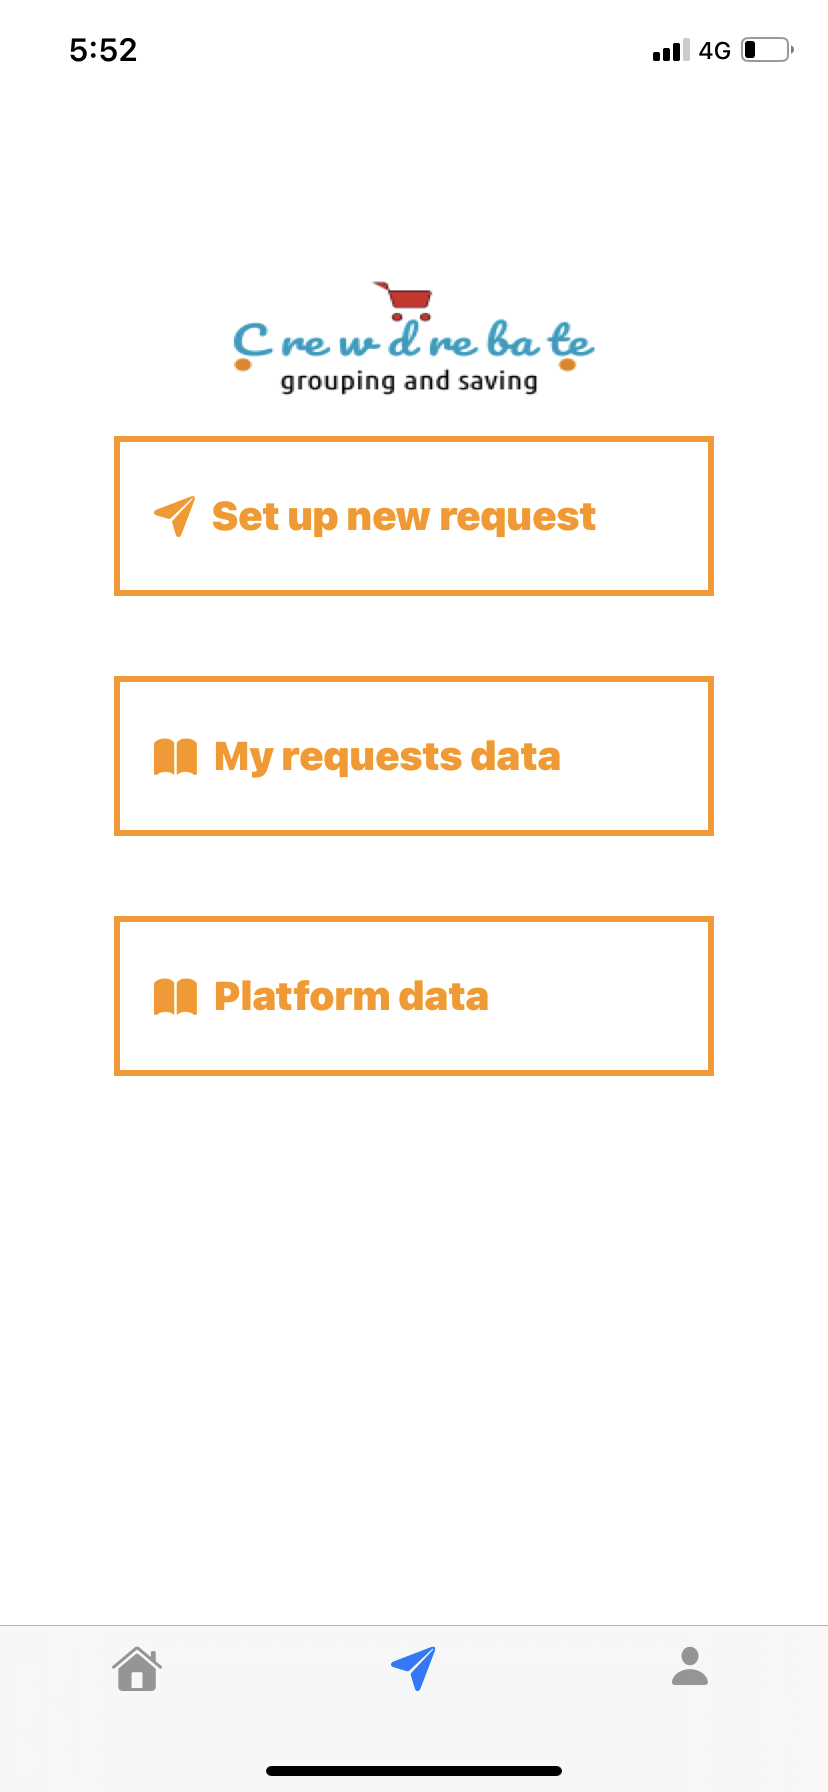
\includegraphics{../figure/request 1.png}}
		\label{fig:request1}}
	\subfigure[][{Fill in information}]{
		\scalebox{0.09}[0.09]{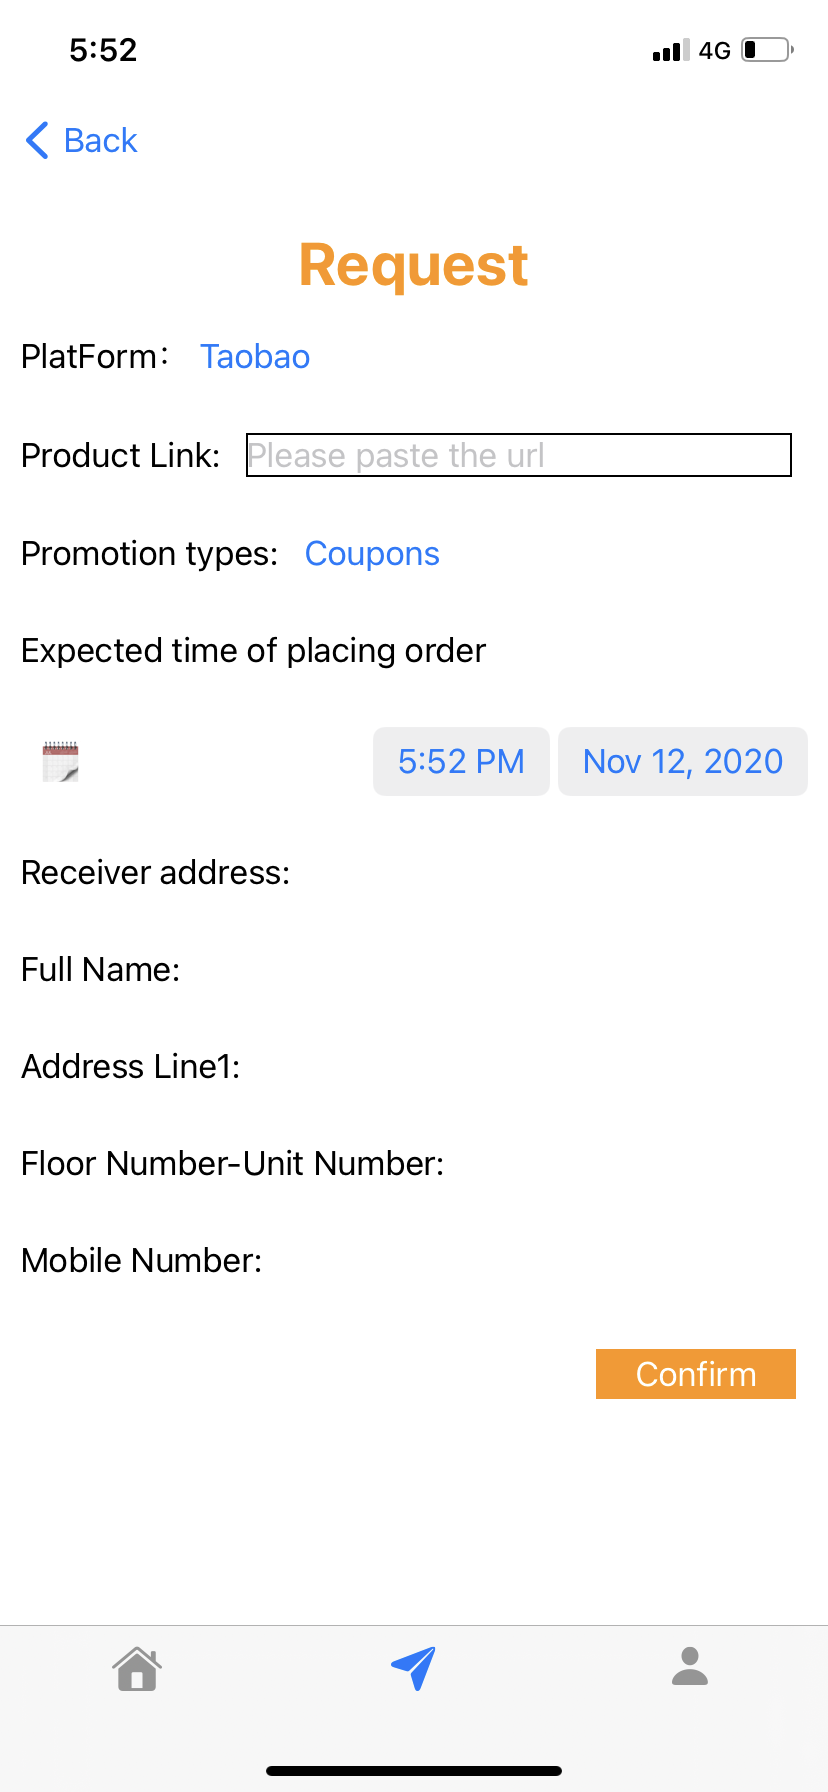
\includegraphics{../figure/request 2.png}}
		\label{fig:request2}}
	\subfigure[][{Information confirm}]{
		\scalebox{0.09}[0.09]{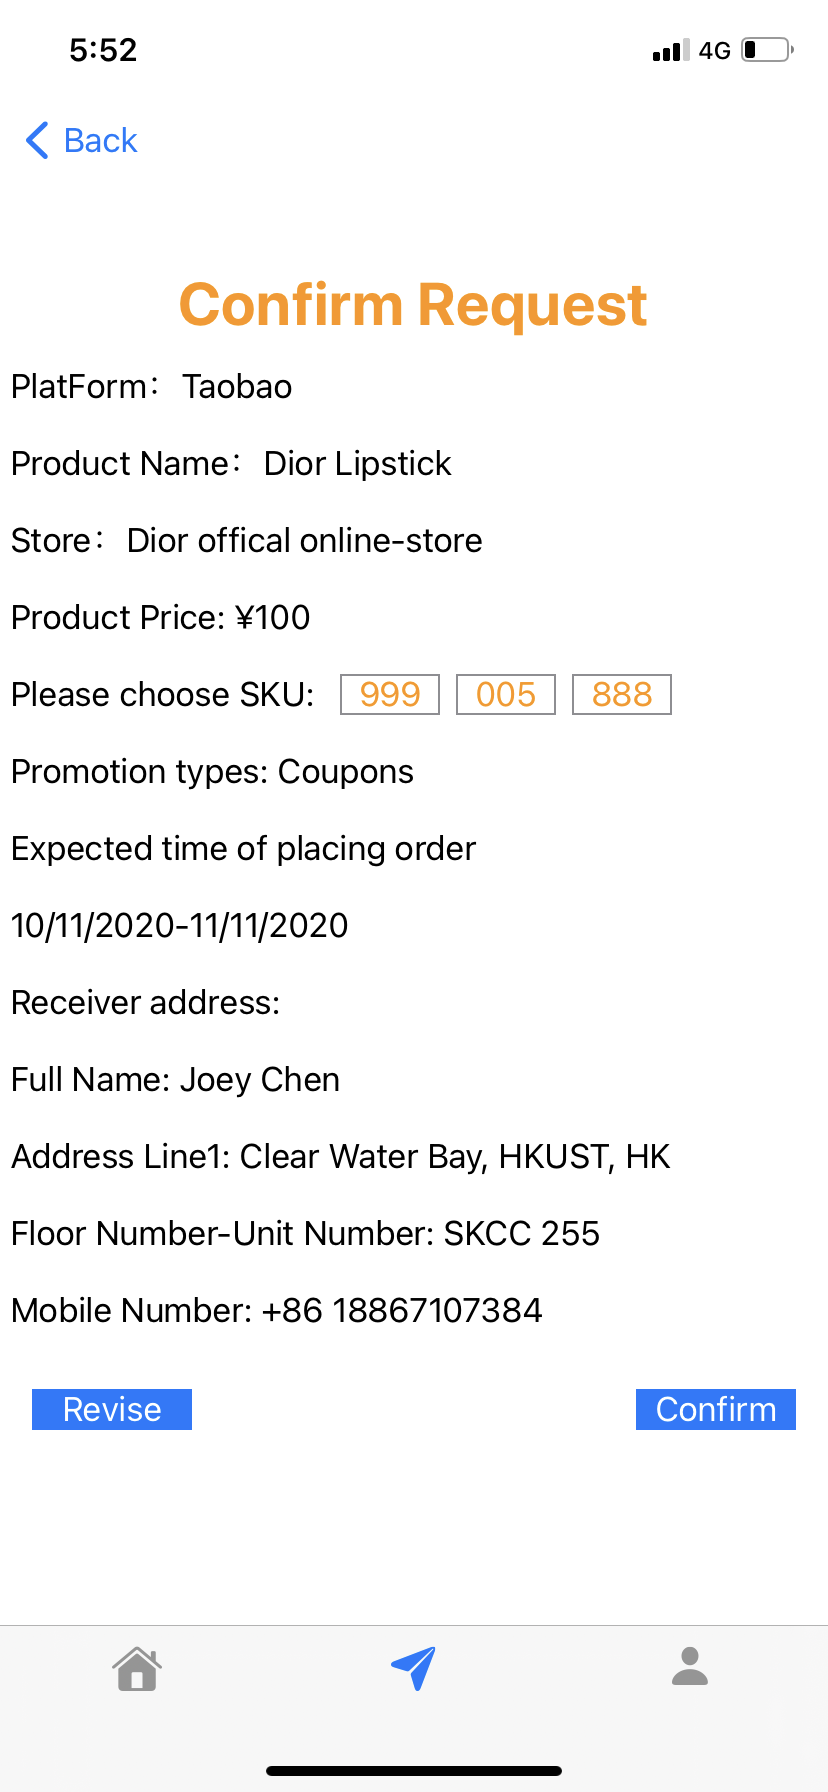
\includegraphics{../figure/request 3.png}}
		\label{fig:request3}}
	\caption{The flowchart of ``Set up a request''.}\vspace{-3ex}
	\label{fig:motivation}
\end{figure}

\textbf{As a regular user} completes the registration on our platform, has the certain product intent to buy, and clicks on the Set up new request button, as shown in Figure~\ref{fig:request1}, she/he would enter the page which guides her/him to fill in the following information in Figure~\ref{fig:request2}. The user needs to select the e-commerce platform she/he wishes to order from. In order to simplify the user's task and to prevent the platform from placing the wrong order of product, the user need to copy the URL link of the product he wants to buy, and the platform will automatically crawl the product information such as price, store, promotions, etc. If there is more than one Stock Keeping Unit SKU~\cite{SKU} for a product, we also crawl to all the SKU information and ask the user to make a choice. Next, the user needs to select the type of promotions he wants to participate in, such as whether to enjoy the coupons or to receive more free samples, and the time slot she/he wants the platform to place the order. Finally, the user fills in the delivery address. After confirming the final information twice shown in Figure~\ref{fig:request3}, the platform will start to deal with the request at the time specified by the user.

\subsection{Scenarios 2: Check request status and data}

\begin{figure}[t!] \vspace{-1.5ex}
	\subfigure[][{Status of requests}]{
		\scalebox{0.13}[0.13]{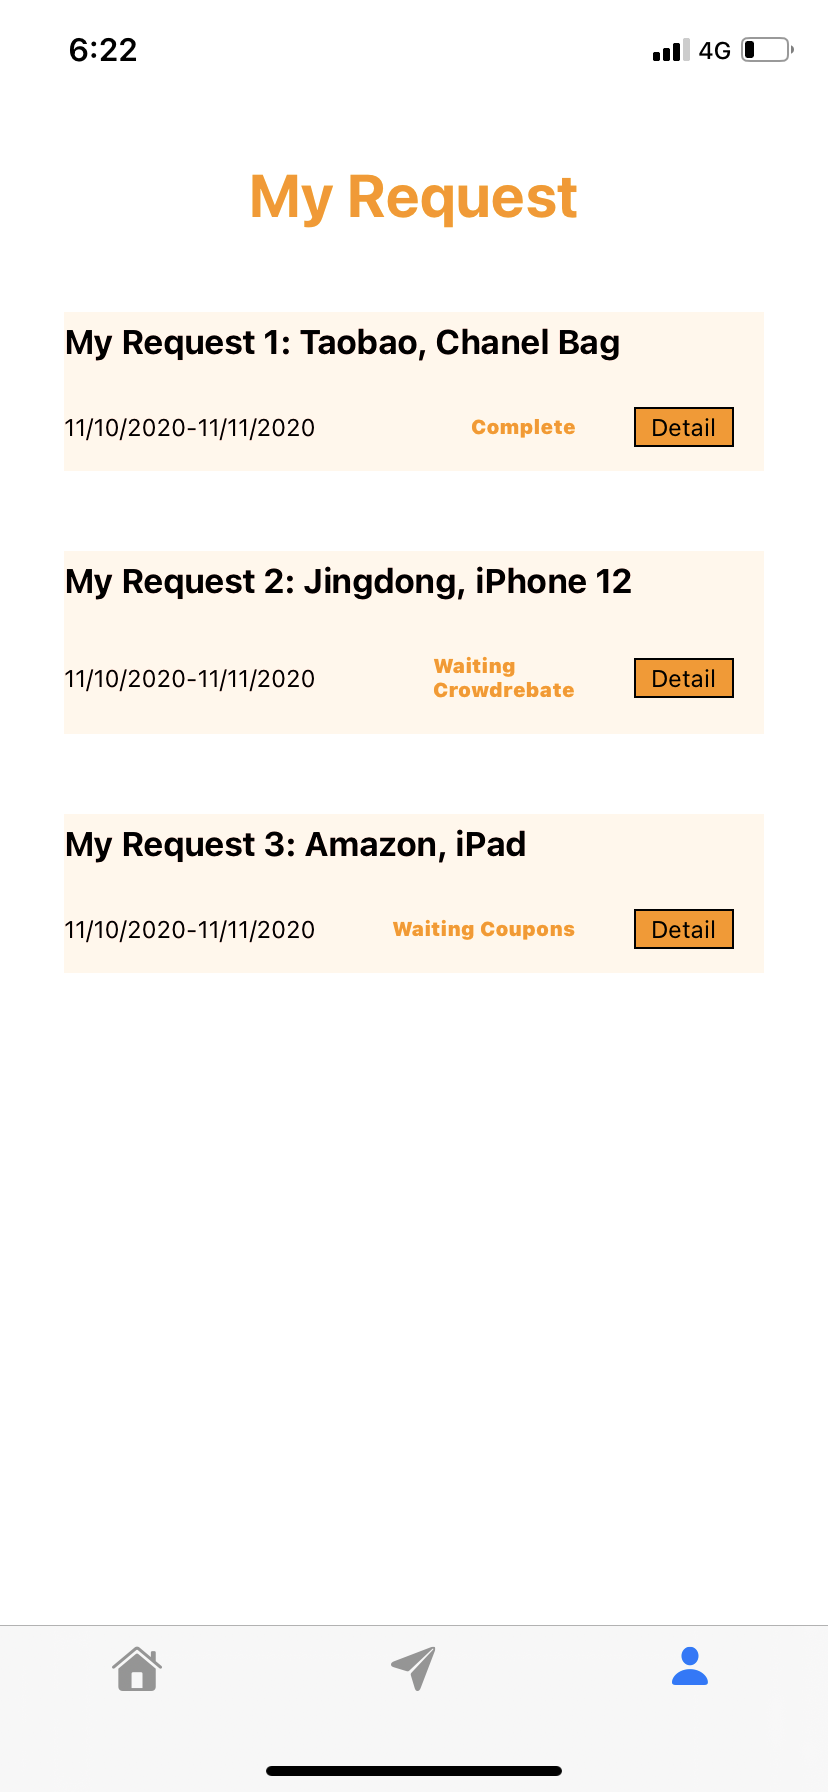
\includegraphics{../figure/check 1.png}}
		\label{fig:check1}}
	\subfigure[][{Personal data}]{
		\scalebox{0.13}[0.13]{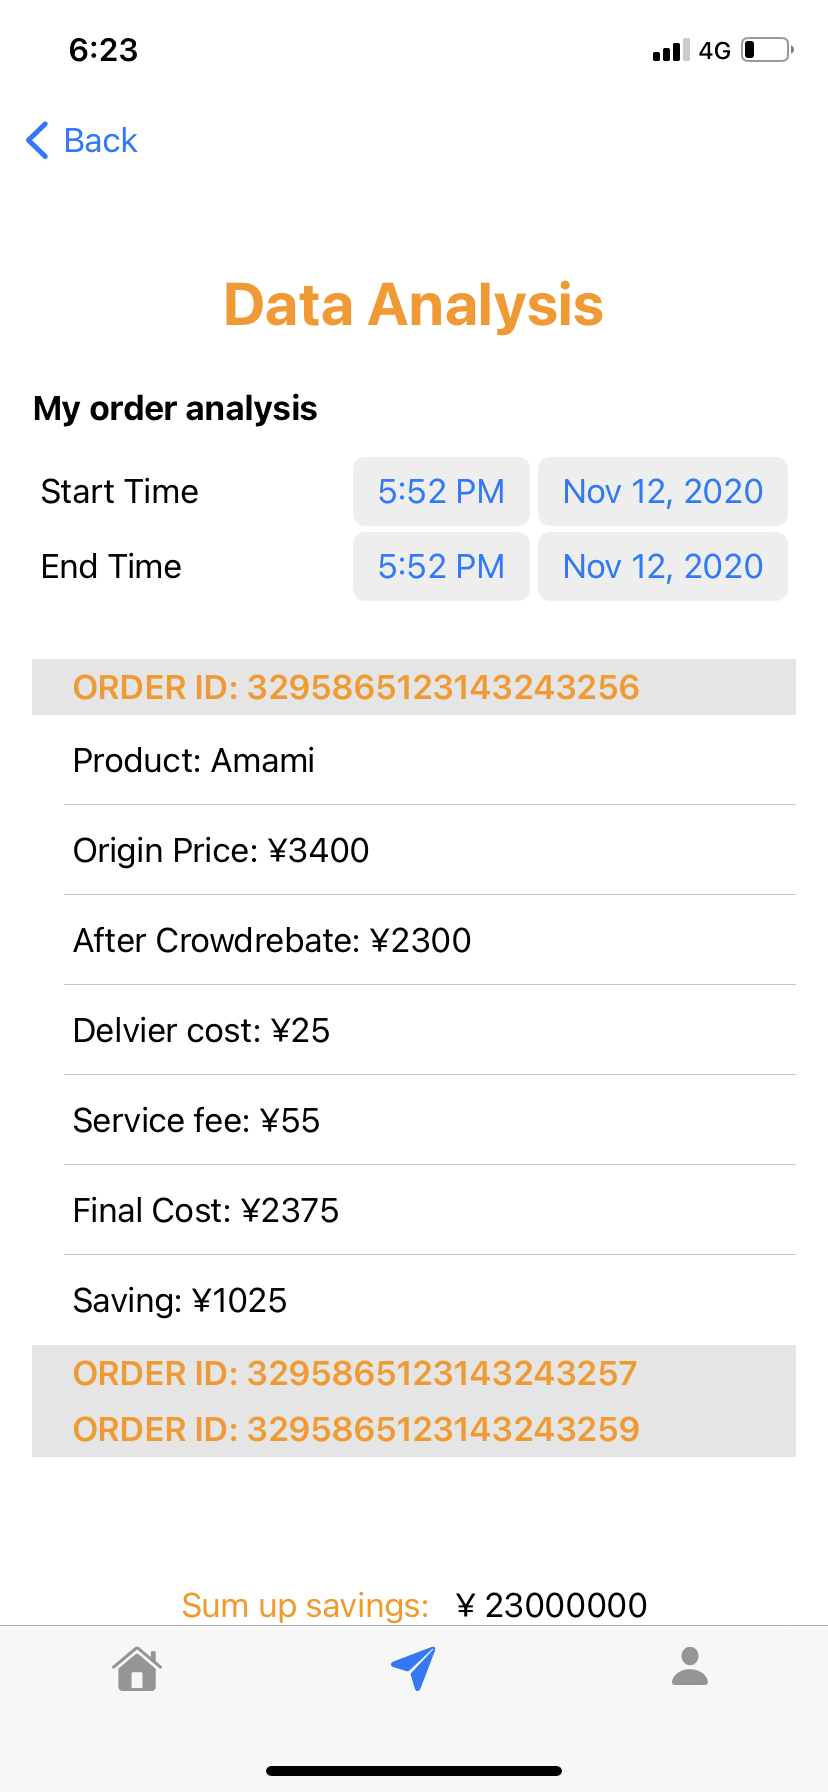
\includegraphics{../figure/check 2.png}}
		\label{fig:check2}}
	\caption{View status of requests and personal data".}\vspace{-3ex}
	\label{fig:check}
\end{figure}

After completing to set up a request, the user can check all the requests she/he made on our platform on the personal page~\ref{fig:check1} and the status of each request, such as whether the order has been placed, and whether the product has been sent to the warehouse, etc.

Note that, if the user has interest in the data of order, she/he can also see specific data for each request in the My request data page~\ref{fig:check2}, like the original price, the price after the platform placed the order for them, the shipping cost, the platform's service charge, and the savings after deducting various costs. The user also can choose to see the sum of the data over a period of time.

\subsection{Scenarios 3: View Top deals and top products}

\begin{figure}[t!] \vspace{-1.5ex}
	\subfigure[][{Today's deals}]{
		\scalebox{0.13}[0.13]{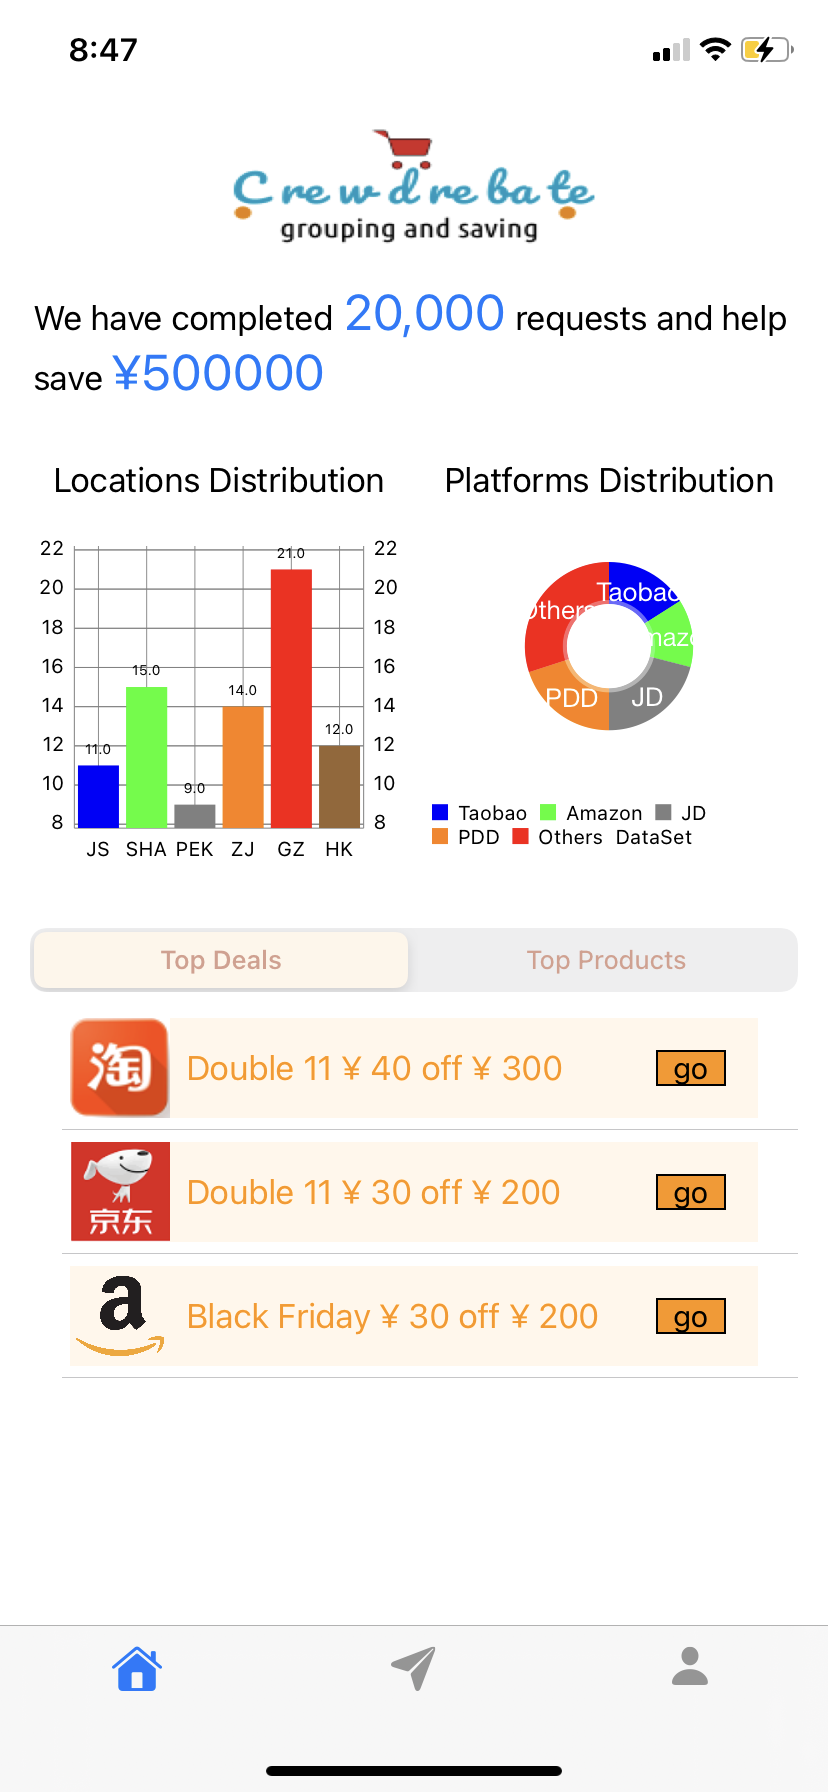
\includegraphics{../figure/home1.png}}
		\label{fig:home1}}
	\subfigure[][{Personalized recommendations}]{
		\scalebox{0.13}[0.13]{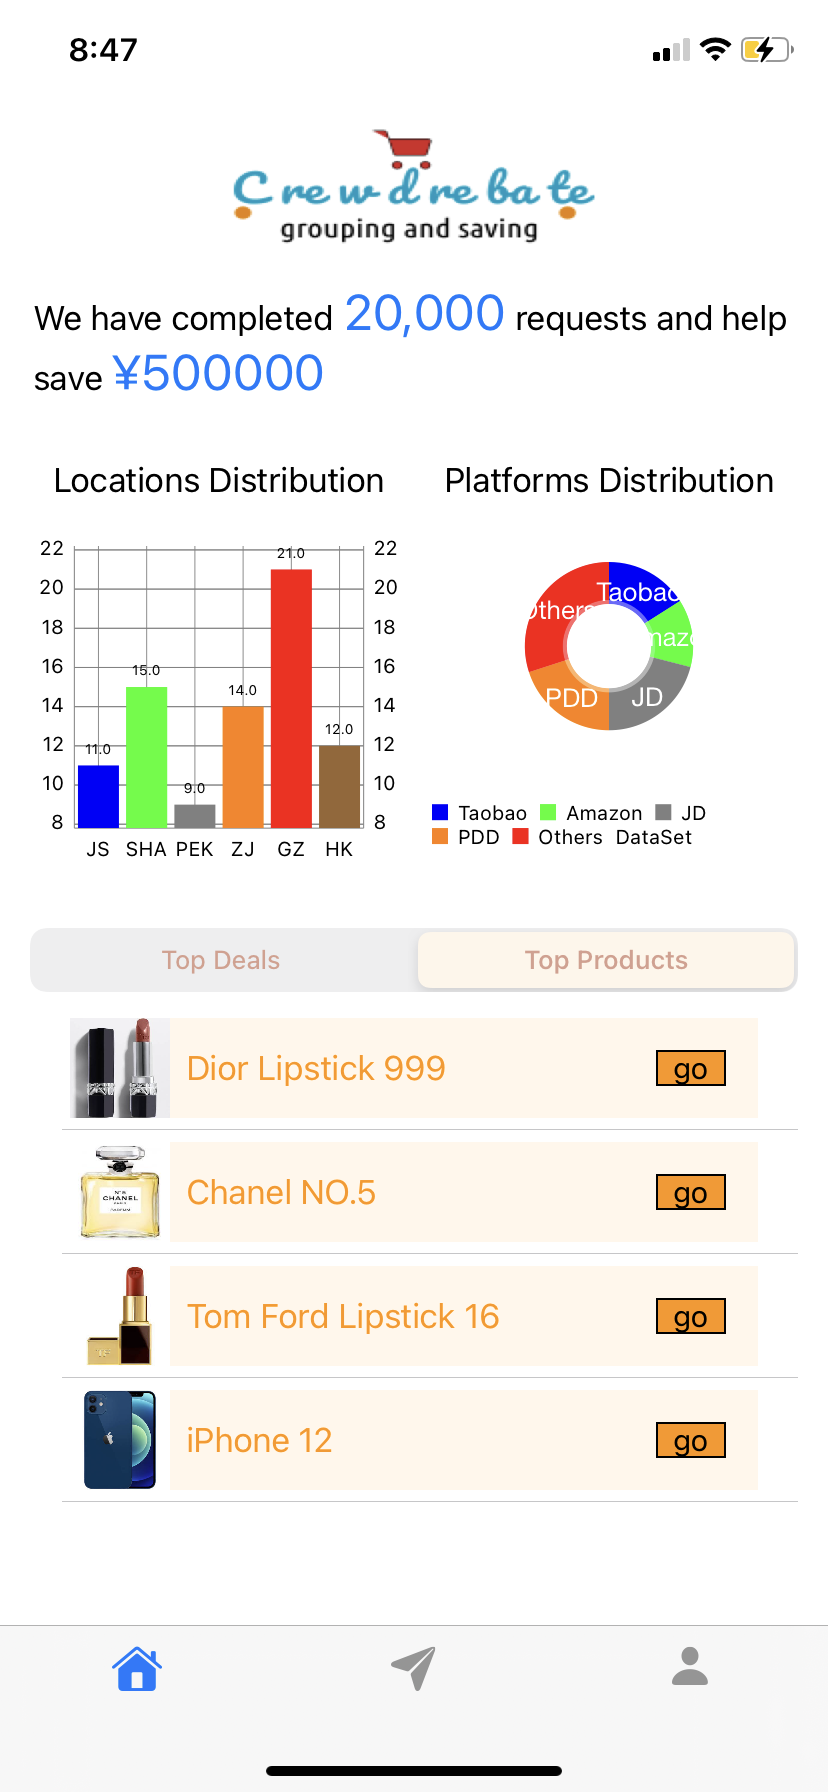
\includegraphics{../figure/home2.png}}
		\label{fig:home2}}
	\caption{View Today's deals and personalized recommendations.}\vspace{-3ex}
	\label{fig:home}
\end{figure}
When user are not sure about recent promotions of e-commerce platforms, she/he can use the home page to see our daily updates of platforms' top deals to save time~\ref{fig:home1}. While having no clear shopping target, the user can view the top products that our crowdrebate platform makes personalized recommendations based on the previous purchase data~\ref{fig:home2}.

\subsection{Scenarios 4: Dashboard of data}

\textbf{As teammates} of the Crowdrebate platform or \textbf{our cooperation partners}, in addition to the basic operations mentioned above, they can also carry out the following functions:

\begin{figure}[t!] \vspace{-1.5ex}
	\subfigure[][{Dashboard of crowdrebate data}]{
		\scalebox{0.13}[0.13]{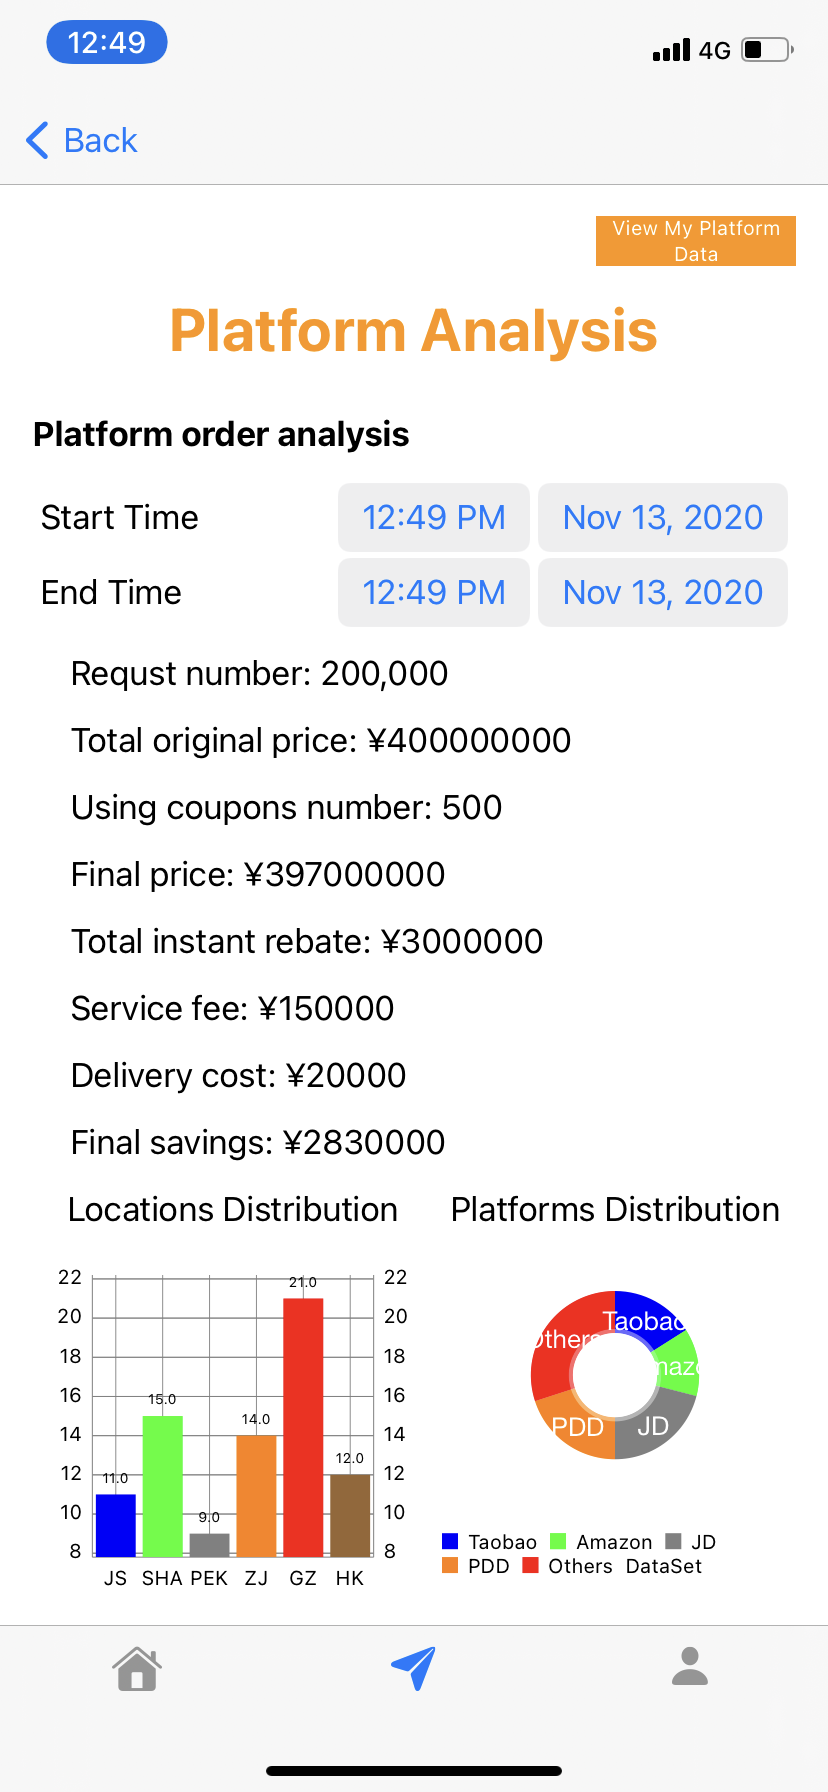
\includegraphics{../figure/data1.png}}
		\label{fig:data1}}
	\subfigure[][{Dashboard of cooperator data}]{
		\scalebox{0.13}[0.13]{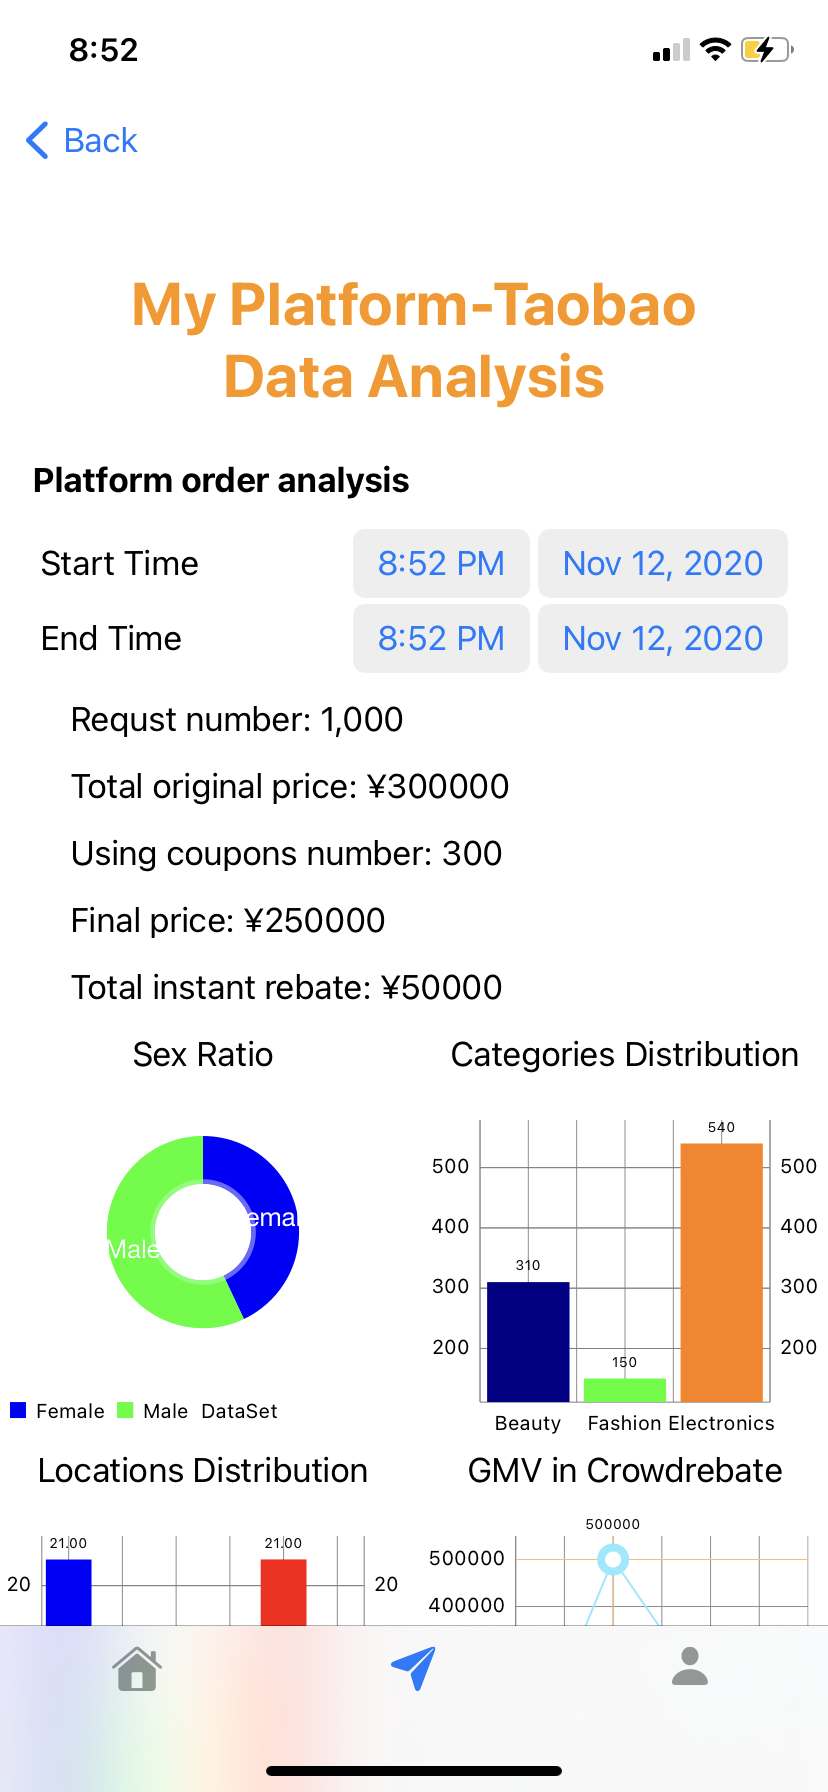
\includegraphics{../figure/data2.png}}
		\label{fig:data2}}
	\caption{Dashboard of data.}\vspace{-3ex}
	\label{data}
\end{figure}

Without being interfered with the user privacy, our platform staffs can enter the third button Platform data~\ref{fig:request1}, where they will be able to see a dashboard of data related to the whole platform, such as how many orders we have received, how many coupons we have used, how much money we have helped users to save, the distribution of our users by regions, and the distribution of platforms they like to launch request~\ref{fig:data1}.

As for our cooperation partners of e-commerce platforms, they can see a dashboard of data related to their platforms. For example, as Taobao cooperators, they can see how many of the requests initiated by our platform users are from Taobao, the distribution of categories they like to buy, the ratio of sex, etc~\ref{fig:data2}. This dashboard of data will help our partners to gain a more practical understanding of user preferences, design coupons, and reach a win-win collaboration mechanism.
